\section{Additional Results}
\label{app:more}

This appendix gives the full results for Sections~\ref{sec:results}
and~\ref{sec:mechanism}. Figure~\ref{fig:shuffle} and Table~\ref{tab:fshuffle}
give the frontier judges on the word-shuffled essays. Figure~\ref{fig:guess}
and Table~\ref{tab:blame} show how often each model is named and how accurate
each judge is on others' text. Table~\ref{tab:naming} gives how often each
judge names Claude and GPT, with false-alarm rates, and Table~\ref{tab:anchor}
repeats the lineup results with the lineups in listed order removed and with
the self-advantage stratified by position. Tables~\ref{tab:fxgenre}
and~\ref{tab:fxsplit} split the API texts by genre and by whether a prompt was
shared with the chat-app essays, and Table~\ref{tab:shared} compares the two
text sets on the shared prompts with intervals. Table~\ref{tab:owyesno} gives
the open-weight judges in the yes/no format, including the answer-first
condition, Table~\ref{tab:owsingle} gives them one text at a time,
Table~\ref{tab:genre} breaks the open-weight results down by genre, and
Table~\ref{tab:owlik} reports what the open-weight judges' likelihoods contain
and whether their claims follow them.

\paragraph{Similarity of the named model to the text} One text at a time, the
model a judge names is the one whose average style is closest to the text in
33.9\% of judgments for function words, 30.6\% for character $n$-grams and
30.3\% for word $n$-grams, compared with 31.5\%, 28.7\% and 29.1\% under random
reassignment.

\paragraph{Prompts used by the likelihood tests} The tests compare texts
within a prompt. In the lineup they use 61 to 96 prompts per judge, but five of the six tests in the
other two formats use 34 or fewer, because the judges claim nearly all or
nearly none of the texts, so those five cannot exclude a moderate effect.

\paragraph{Shuffled lineup} The instruction did not mention the reordering.
Every reasoning trace returned by Gemini and Grok (38 each) describes the
essays as scrambled, and every answered lineup assigns each of the five names
once.

\begin{figure}[!ht]
\centering
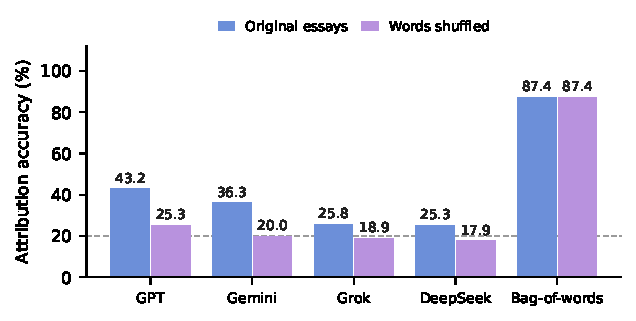
\includegraphics[width=0.8\linewidth]{figures/shuffle.pdf}
\caption{Lineup accuracy of four frontier judges on the chat-app essays in
their original form and with the words of each essay shuffled, compared with
a bag-of-words classifier on the same essays. With shuffled words the judges'
accuracy is between \FSDeepSeekOverall{} and \FSGPTOverall{}, close to chance
(dashed line). The classifier does not use word order, so its two bars are
equal by construction. Claude is omitted because its provider refused all
shuffled lineups, and Gemini's shuffled bar is based on 24 of its 38
lineups.}
\label{fig:shuffle}
\end{figure}

% Shuffled-lineup table, corrected (issue I15). Numbers hard-coded; recomputed from
% repo/results/revision/frontier/shuffle_lineup.jsonl by work/verify-I15/t8.py.
% SAMPLE RULE (applies to every cell of every row): the 24 prompts on which all
% four answering judges (GPT, Gemini, Grok, DeepSeek) returned a complete,
% parseable shuffled lineup (ok = true). That is 96 lineups and 480 judgments.
%   Self   = judge names itself on its own essay, k/24
%   Peer   = the three other answering judges name it on its essay, k/72
%            (Claude has no shuffled judgments, so it is not a peer)
%   FA     = judge names itself on the four essays it did not write, k/96
%   Self-adv. = Self - Peer; percentile bootstrap over the 24 prompts
%   Hit-FA = Self - FA (now equals the printed Self minus the printed FA)
% Counts: GPT 9/24, 18/72, 15/96; Gemini 5/24, 13/72, 19/96;
%         Grok 2/24, 10/72, 22/96; DeepSeek 3/24, 7/72, 21/96.
% Exact randomisation p (uncorrected / Holm over four judges):
%   Self-adv.: GPT 0.31/1.00, Gemini 1.00/1.00, Grok 0.67/1.00, DeepSeek 1.00/1.00
%   Hit-FA:    GPT 0.041/0.16, Gemini 1.00/1.00, Grok 0.20/0.61, DeepSeek 0.45/0.91
% The earlier version took Self and Peer from these 24 prompts but FA and Hit-FA
% from all 38 (GPT 17.1%, +14.5; Grok 21.7%, -8.6; DeepSeek 21.7%, -8.6).
% Original (last column) is unchanged: unshuffled essays, all 38 prompts, four peers.
\begin{table}[t]
\centering\small
\setlength\tabcolsep{2.5pt}
\begin{adjustbox}{max width=\linewidth}
\begin{tabular}{l rrr l r r}
\toprule
Judge & Self & Peer & FA & Self-adv. [95\% CI] & Hit$-$FA & Original \\
\midrule
GPT & 37.5\% & 25.0\% & 15.6\% & +12.5 [$-$12.5, +38.9] & +21.9 & \GPTAdvLineup \\
Claude & \multicolumn{5}{c}{\emph{refused every lineup}} & \ClaudeAdvLineup \\
Gemini & 20.8\% & 18.1\% & 19.8\% & +2.8 [$-$15.3, +22.2] & +1.0 & \GeminiAdvLineup \\
Grok & 8.3\% & 13.9\% & 22.9\% & $-$5.6 [$-$16.7, +6.9] & $-$14.6 & \GrokAdvLineup \\
DeepSeek & 12.5\% & 9.7\% & 21.9\% & +2.8 [$-$11.1, +19.4] & $-$9.4 & \DeepSeekAdvLineup \\
\bottomrule
\end{tabular}
\end{adjustbox}
\caption{The chat-app lineup repeated with every essay's words shuffled. All columns use the 24 prompts on which GPT, Gemini, Grok and DeepSeek each returned a complete lineup (Gemini returned none for 14 of the 38). Columns as in Table~\ref{tab:frontier}, with the peer baseline taken over the three other answering judges; Original is the self-advantage on the unshuffled essays (all 38 prompts, four peers). Claude's provider refused all 38 of Claude's shuffled lineups, so Claude has no judgments here and is not a peer, although its essays stayed in every lineup. No value is significant after Holm correction over the four judges (smallest corrected $p=0.16$, for GPT's Hit$-$FA).}
\label{tab:fshuffle}
\end{table}


\begin{figure}[!ht]
\centering
\begin{subfigure}[b]{0.49\linewidth}\centering
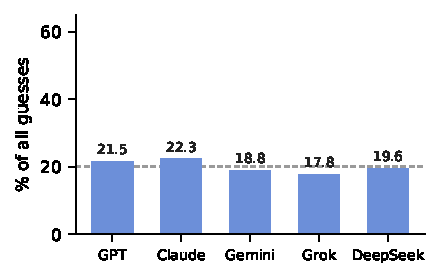
\includegraphics[width=\linewidth]{figures/guess_lineup.pdf}
\caption{Lineup}\label{fig:guess-lineup}
\end{subfigure}\hfill
\begin{subfigure}[b]{0.49\linewidth}\centering
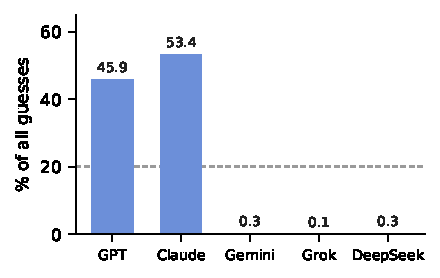
\includegraphics[width=\linewidth]{figures/guess_single.pdf}
\caption{One text at a time}\label{fig:guess-single}
\end{subfigure}
\caption{Share of the 950 attributions on the chat-app essays that name each
model. In the lineup the shares are close to uniform. One text at a time, GPT
and Claude receive \SingleConcentration{} of attributions and Gemini, Grok and
DeepSeek almost none. The dashed line marks a uniform distribution (20\%).}
\label{fig:guess}
\end{figure}

\begin{figure}[!ht]
\centering
\begin{subfigure}[b]{0.49\linewidth}\centering
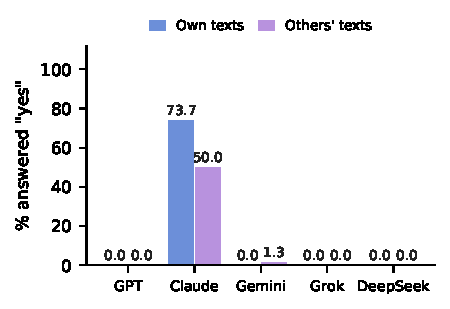
\includegraphics[width=\linewidth]{figures/yes_frontier.pdf}
\caption{Frontier judges, chat-app essays}\label{fig:yes-frontier}
\end{subfigure}\hfill
\begin{subfigure}[b]{0.49\linewidth}\centering
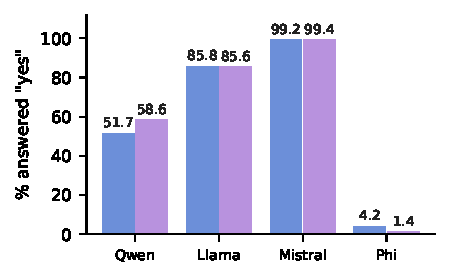
\includegraphics[width=\linewidth]{figures/yes_open.pdf}
\caption{Open-weight judges}\label{fig:yes-open}
\end{subfigure}
\caption{Share of texts for which a judge answers ``yes'' to ``Did you write
this text?'', separately for its own texts and for other models' texts.
(a) GPT, Grok and DeepSeek answer no for every essay; Claude is the only judge
that answers yes for its own essays. (b) Mistral answers yes for almost every
text and Phi for almost none, regardless of authorship.}
\label{fig:yes}
\end{figure}

\begin{table}[t]
\centering\small
\setlength\tabcolsep{3pt}
\begin{adjustbox}{max width=\linewidth}
\begin{tabular}{l rr rr rr}
\toprule
 & \multicolumn{2}{c}{Share of guesses} & \multicolumn{2}{c}{Non-self acc.} & \multicolumn{2}{c}{Overall acc.} \\
\cmidrule(lr){2-3}\cmidrule(lr){4-5}\cmidrule(lr){6-7}
Model & Lineup & Single & Lineup & Single & Lineup & Single \\
\midrule
GPT & \GPTBlameLineup & \GPTBlameSingle & \GPTNonSelfLineup & \GPTNonSelfSingle & \GPTOverallLineup & \GPTOverallSingle \\
Claude & \ClaudeBlameLineup & \ClaudeBlameSingle & \ClaudeNonSelfLineup & \ClaudeNonSelfSingle & \ClaudeOverallLineup & \ClaudeOverallSingle \\
Gemini & \GeminiBlameLineup & \GeminiBlameSingle & \GeminiNonSelfLineup & \GeminiNonSelfSingle & \GeminiOverallLineup & \GeminiOverallSingle \\
Grok & \GrokBlameLineup & \GrokBlameSingle & \GrokNonSelfLineup & \GrokNonSelfSingle & \GrokOverallLineup & \GrokOverallSingle \\
DeepSeek & \DeepSeekBlameLineup & \DeepSeekBlameSingle & \DeepSeekNonSelfLineup & \DeepSeekNonSelfSingle & \DeepSeekOverallLineup & \DeepSeekOverallSingle \\
\bottomrule
\end{tabular}
\end{adjustbox}
\caption{Frontier judges, chat-app essays. Share of guesses: how often each model is
named, over all five judges' 950 judgments per format. Non-self accuracy: the
judge's accuracy on the 152 texts it did not write; overall: on all 190
(chance 20\%). The lineup spreads guesses evenly; one text at a time, GPT and
Claude receive almost all of them.}
\label{tab:blame}
\label{tab:nonself}
\end{table}

\begin{table}[t]
\centering\small
\setlength\tabcolsep{4pt}
\begin{adjustbox}{max width=\linewidth}
\begin{tabular}{l rr rr rr}
\toprule
 & \multicolumn{2}{c}{Chat-app, lineup} & \multicolumn{2}{c}{Chat-app, one text} & \multicolumn{2}{c}{API, lineup} \\
\cmidrule(lr){2-3}\cmidrule(lr){4-5}\cmidrule(lr){6-7}
Judge & Hit & False alarm & Hit & False alarm & Hit & False alarm \\
\midrule
\multicolumn{7}{l}{\emph{Naming Claude}} \\
GPT & 84.2 & 4.6 & 97.4 & 25.0 & 48.3 & 13.1 \\
Claude & \textbf{86.8} & \textbf{9.2} & \textbf{86.8} & \textbf{8.6} & \textbf{56.7} & \textbf{12.7} \\
Gemini & 63.2 & 9.2 & 100.0 & 77.6 & 74.2 & 6.5 \\
Grok & 34.2 & 20.4 & 100.0 & 86.8 & 55.0 & 12.7 \\
DeepSeek & 34.2 & 20.4 & 31.6 & 31.6 & 24.2 & 21.2 \\
\midrule
\multicolumn{7}{l}{\emph{Naming GPT}} \\
GPT & \textbf{57.9} & \textbf{10.5} & \textbf{94.7} & \textbf{52.0} & \textbf{19.2} & \textbf{20.4} \\
Claude & 31.6 & 19.7 & 97.4 & 66.4 & 25.8 & 21.9 \\
Gemini & 31.6 & 17.1 & 31.6 & 13.8 & 6.7 & 23.3 \\
Grok & 34.2 & 16.4 & 34.2 & 4.6 & 14.2 & 21.7 \\
DeepSeek & 23.7 & 25.7 & 81.6 & 65.1 & 13.3 & 27.3 \\
\bottomrule
\end{tabular}
\end{adjustbox}
\caption{How often each frontier judge names Claude and names GPT (\%). Hit: on the texts that model wrote (38 chat-app essays, 120 API texts). False alarm: on the texts of the other four models (152 and 480). Bold rows are the judge's own texts and repeat the self-naming and false-alarm rates of Tables~\ref{tab:frontier} and~\ref{tab:frontier120}. The mean of the four other hit rates in a block is the peer baseline. The chat-app hit rates are the Claude and GPT columns of Figure~\ref{fig:naming}.}
\label{tab:naming}
\end{table}

\begin{table}[t]
\centering\small
\setlength\tabcolsep{5pt}
\begin{adjustbox}{max width=\linewidth}
\begin{tabular}{l rr}
\toprule
 & Chat-app essays & API texts \\
\midrule
Lineups that use each name once & 162/190 (85.3\%) & 539/600 (89.8\%) \\
\midrule
\multicolumn{3}{l}{\emph{Attribution accuracy, all five judges}} \\
\quad Answers in the listed order of the names & 105/190 (55.3\%) & 275/600 (45.8\%) \\
\quad Answers in the other four orders & 215/760 (28.3\%) & 615/2{,}400 (25.6\%) \\
\midrule
\multicolumn{3}{l}{\emph{Self-advantage of Claude (points)}} \\
\quad As printed, all lineups & +32.9 & +6.2 \\
\quad Stratified by position of the text & +34.1 & +6.2 \\
\quad Listed-order lineups removed & +35.9 & +2.9 \\
\midrule
\multicolumn{3}{l}{\emph{Self-advantage of GPT (points)}} \\
\quad As printed, all lineups & +27.6 & +4.2 \\
\quad Stratified by position of the text & +26.7 & +4.2 \\
\quad Listed-order lineups removed & +27.8 & +0.5 \\
\bottomrule
\end{tabular}
\end{adjustbox}
\caption{Lineup design and the frontier results. The answers to a prompt appear in one of five orders, the rotations of the order in which the instructions list the candidate names, so in one fifth of the lineups the answers follow the listed order. Judges tend to assign the names in that order, and accuracy is about twice as high in those lineups. Every judge sees each model's answer in each position equally often, so the effect raises the self-naming rate and the peer baseline together. The self-advantages of Claude and GPT on the chat-app essays change by about 3 points or less when they are computed within each position of the text and averaged, or when the listed-order lineups are removed. On the API texts positions are fully balanced within each judge, so stratifying leaves the self-advantage unchanged. First row: lineups in which the judge assigns each of the five names to one answer, although the instructions allow repeats.}
\label{tab:anchor}
\end{table}

\begin{table}[t]
\centering\small
\setlength\tabcolsep{3pt}
\begin{adjustbox}{max width=\linewidth}
\begin{tabular}{l rr rr rr rr}
\toprule
 & \multicolumn{2}{c}{Prose} & \multicolumn{2}{c}{Code} & \multicolumn{2}{c}{Short} & \multicolumn{2}{c}{Math} \\
\cmidrule(lr){2-3}\cmidrule(lr){4-5}\cmidrule(lr){6-7}\cmidrule(lr){8-9}
Judge & Adv. & Disc. & Adv. & Disc. & Adv. & Disc. & Adv. & Disc. \\
\midrule
\multicolumn{9}{l}{\emph{Lineup}} \\
GPT & \FXGPTLineupProseAdv & \FXGPTLineupProseDisc & \FXGPTLineupCodeAdv & \FXGPTLineupCodeDisc & \FXGPTLineupShortAdv & \FXGPTLineupShortDisc & \FXGPTLineupMathAdv & \FXGPTLineupMathDisc \\
Claude & \FXClaudeLineupProseAdv & \FXClaudeLineupProseDisc & \FXClaudeLineupCodeAdv & \FXClaudeLineupCodeDisc & \FXClaudeLineupShortAdv & \FXClaudeLineupShortDisc & \FXClaudeLineupMathAdv & \FXClaudeLineupMathDisc \\
Gemini & \FXGeminiLineupProseAdv & \FXGeminiLineupProseDisc & \FXGeminiLineupCodeAdv & \FXGeminiLineupCodeDisc & \FXGeminiLineupShortAdv & \FXGeminiLineupShortDisc & \FXGeminiLineupMathAdv & \FXGeminiLineupMathDisc \\
Grok & \FXGrokLineupProseAdv & \FXGrokLineupProseDisc & \FXGrokLineupCodeAdv & \FXGrokLineupCodeDisc & \FXGrokLineupShortAdv & \FXGrokLineupShortDisc & \FXGrokLineupMathAdv & \FXGrokLineupMathDisc \\
DeepSeek & \FXDeepSeekLineupProseAdv & \FXDeepSeekLineupProseDisc & \FXDeepSeekLineupCodeAdv & \FXDeepSeekLineupCodeDisc & \FXDeepSeekLineupShortAdv & \FXDeepSeekLineupShortDisc & \FXDeepSeekLineupMathAdv & \FXDeepSeekLineupMathDisc \\
\midrule
\multicolumn{9}{l}{\emph{One text at a time}} \\
GPT & \FXGPTSingleProseAdv & \FXGPTSingleProseDisc & \FXGPTSingleCodeAdv & \FXGPTSingleCodeDisc & \FXGPTSingleShortAdv & \FXGPTSingleShortDisc & \FXGPTSingleMathAdv & \FXGPTSingleMathDisc \\
Claude & \FXClaudeSingleProseAdv & \FXClaudeSingleProseDisc & \FXClaudeSingleCodeAdv & \FXClaudeSingleCodeDisc & \FXClaudeSingleShortAdv & \FXClaudeSingleShortDisc & \FXClaudeSingleMathAdv & \FXClaudeSingleMathDisc \\
Gemini & \FXGeminiSingleProseAdv & \FXGeminiSingleProseDisc & \FXGeminiSingleCodeAdv & \FXGeminiSingleCodeDisc & \FXGeminiSingleShortAdv & \FXGeminiSingleShortDisc & \FXGeminiSingleMathAdv & \FXGeminiSingleMathDisc \\
Grok & \FXGrokSingleProseAdv & \FXGrokSingleProseDisc & \FXGrokSingleCodeAdv & \FXGrokSingleCodeDisc & \FXGrokSingleShortAdv & \FXGrokSingleShortDisc & \FXGrokSingleMathAdv & \FXGrokSingleMathDisc \\
DeepSeek & \FXDeepSeekSingleProseAdv & \FXDeepSeekSingleProseDisc & \FXDeepSeekSingleCodeAdv & \FXDeepSeekSingleCodeDisc & \FXDeepSeekSingleShortAdv & \FXDeepSeekSingleShortDisc & \FXDeepSeekSingleMathAdv & \FXDeepSeekSingleMathDisc \\
\bottomrule
\end{tabular}
\end{adjustbox}
\caption{Frontier judges on the API texts, by genre: self-advantage (Adv.) and hit minus
false-alarm rate (Disc.), in points, for each judge. Per judge, 60 own texts
in prose and 20 in each other genre. Claude's discrimination is largest on
prose and absent on math; Grok's is largest on code.}
\label{tab:fxgenre}
\end{table}

\begin{table}[t]
\centering\small
\setlength\tabcolsep{3pt}
\begin{adjustbox}{max width=\linewidth}
\begin{tabular}{l rrrr rrrr}
\toprule
 & \multicolumn{4}{c}{38 shared prompts} & \multicolumn{4}{c}{82 new prompts} \\
\cmidrule(lr){2-5}\cmidrule(lr){6-9}
Judge & Self & Peer & Adv. & Disc. & Self & Peer & Adv. & Disc. \\
\midrule
GPT & \FXOldGPTLineupSelf & \FXOldGPTLineupPeer & \FXOldGPTLineupAdv & \FXOldGPTLineupDisc & \FXNewGPTLineupSelf & \FXNewGPTLineupPeer & \FXNewGPTLineupAdv & \FXNewGPTLineupDisc \\
Claude & \FXOldClaudeLineupSelf & \FXOldClaudeLineupPeer & \FXOldClaudeLineupAdv & \FXOldClaudeLineupDisc & \FXNewClaudeLineupSelf & \FXNewClaudeLineupPeer & \FXNewClaudeLineupAdv & \FXNewClaudeLineupDisc \\
Gemini & \FXOldGeminiLineupSelf & \FXOldGeminiLineupPeer & \FXOldGeminiLineupAdv & \FXOldGeminiLineupDisc & \FXNewGeminiLineupSelf & \FXNewGeminiLineupPeer & \FXNewGeminiLineupAdv & \FXNewGeminiLineupDisc \\
Grok & \FXOldGrokLineupSelf & \FXOldGrokLineupPeer & \FXOldGrokLineupAdv & \FXOldGrokLineupDisc & \FXNewGrokLineupSelf & \FXNewGrokLineupPeer & \FXNewGrokLineupAdv & \FXNewGrokLineupDisc \\
DeepSeek & \FXOldDeepSeekLineupSelf & \FXOldDeepSeekLineupPeer & \FXOldDeepSeekLineupAdv & \FXOldDeepSeekLineupDisc & \FXNewDeepSeekLineupSelf & \FXNewDeepSeekLineupPeer & \FXNewDeepSeekLineupAdv & \FXNewDeepSeekLineupDisc \\
\bottomrule
\end{tabular}
\end{adjustbox}
\caption{Frontier judges on the API texts, lineup, split into the 38 prompts shared with the
chat-app essays and the 82 added for this study. On the shared prompts
Claude's self-naming rate (\FXOldClaudeLineupSelf) is close to its chat-app
rate (\ClaudeSelfLineup), but its peers now name it almost as often.}
\label{tab:fxsplit}
\end{table}

% Generated by code_council/build_shared.py. Do not edit by hand.
\begin{table}[t]
\centering\footnotesize
\setlength\tabcolsep{3pt}
\begin{adjustbox}{max width=\linewidth}
\begin{tabular}{l lll rrl}
\toprule
 & \multicolumn{3}{c}{Self-advantage} & \multicolumn{3}{c}{Discrimination} \\
\cmidrule(lr){2-4}\cmidrule(lr){5-7}
Judge & Chat-app & API & Difference & Chat-app & API & Difference \\
\midrule
GPT & +27.6 [+10.5, +44.7]$^{*}$ & +12.5 [$-$1.3, +27.6] & +15.1 [$-$8.6, +37.5] & +47.4 & +11.2 & +36.2 [+9.9, +62.5]$^{*}$ \\
Claude & +32.9 [+20.4, +44.1]$^{*}$ & +17.8 [+3.3, +30.9]$^{*}$ & +15.1 [$-$3.9, +33.6] & +77.6 & +73.7 & +3.9 [$-$18.4, +27.0] \\
Gemini & $-$9.9 [$-$23.0, +4.6] & +3.3 [$-$13.2, +21.1] & $-$13.2 [$-$32.2, +5.3] & $-$2.0 & +17.8 & $-$19.7 [$-$42.8, +0.0] \\
Grok & $-$23.7 [$-$32.9, $-$13.8]$^{*}$ & $-$3.9 [$-$19.1, +12.5] & $-$19.7 [$-$36.8, $-$3.3]$^{*}$ & $-$15.1 & +3.3 & $-$18.4 [$-$36.2, $-$2.0]$^{*}$ \\
DeepSeek & $-$0.7 [$-$15.1, +14.5] & $-$2.0 [$-$14.5, +11.2] & +1.3 [$-$18.4, +21.7] & +3.3 & $-$2.0 & +5.3 [$-$14.5, +25.0] \\
\bottomrule
\end{tabular}
\end{adjustbox}
\caption{Frontier judges in the lineup on the 38 prompts that the chat-app essays and the API texts share, in points. Self-advantage is the self-naming rate minus the peer baseline, and discrimination is the self-naming rate minus the false-alarm rate. Difference is the chat-app value minus the API value. Brackets are 95\% bootstrap intervals over prompts (10{,}000 resamples, with the same resampled prompts applied to both text sets), and an asterisk marks an interval that excludes zero. The intervals are not corrected for multiple comparisons. For Claude and GPT the two self-advantages differ by about 15 points and both intervals for the difference include zero. GPT's discrimination is lower on the API texts, and Claude's is almost the same on both sets. Interval endpoints can differ from Table~\ref{tab:frontier} by under one point because the resamples differ.}
\label{tab:shared}
\end{table}


\paragraph{Answer-first condition}
When a judge first answers the prompt and is then asked about either that same
answer or a peer's answer, every judge's AUC is above chance
(Table~\ref{tab:owyesno}). Because the candidate repeats verbatim text already in
the conversation, this condition mainly tests matching within the context
rather than recognition of style. Even so, Llama's AUC is only
\OWLlamaOnPolAUC{}. When the candidate is instead a separately sampled answer
by the judge, Qwen and Phi distinguish it from peers' answers (AUC
\OWQwenOnPolResAUC{} and \OWPhiOnPolResAUC{}, against a mean of
\CXPeerAUCQwen{} and \CXPeerAUCPhi{} when the other three judges are asked
about the same answers). Llama's and Mistral's AUCs are below 0.5
(\OWLlamaOnPolResAUC{} and \OWMistralOnPolResAUC{}), but the other judges rank
these two authors' answers low as well (mean peer AUC \CXPeerAUCLlama{} and
\CXPeerAUCMistral{}), so the low values mostly reflect the author of the text
and say little about the judge.

\begin{table}[t]
\centering\small
\setlength\tabcolsep{4pt}
\begin{adjustbox}{max width=\linewidth}
\begin{tabular}{l rrl rrl rrl}
\toprule
 & \multicolumn{3}{c}{Asked in a fresh conversation} & \multicolumn{3}{c}{After answering: same answer} & \multicolumn{3}{c}{After answering: a new answer} \\
\cmidrule(lr){2-4}\cmidrule(lr){5-7}\cmidrule(lr){8-10}
Judge & Hit & FA & AUC [95\% CI] & Hit & FA & AUC [95\% CI] & Hit & FA & AUC [95\% CI] \\
\midrule
Qwen & \OWQwenBinaryHit & \OWQwenBinaryFA & \OWQwenBinaryAUC{} \OWQwenBinaryAUCCI & \OWQwenOnPolHit & \OWQwenOnPolFA & \OWQwenOnPolAUC{} \OWQwenOnPolAUCCI & \OWQwenOnPolResHit & \OWQwenOnPolResFA & \OWQwenOnPolResAUC{} \OWQwenOnPolResAUCCI \\
Llama & \OWLlamaBinaryHit & \OWLlamaBinaryFA & \OWLlamaBinaryAUC{} \OWLlamaBinaryAUCCI & \OWLlamaOnPolHit & \OWLlamaOnPolFA & \OWLlamaOnPolAUC{} \OWLlamaOnPolAUCCI & \OWLlamaOnPolResHit & \OWLlamaOnPolResFA & \OWLlamaOnPolResAUC{} \OWLlamaOnPolResAUCCI \\
Mistral & \OWMistralBinaryHit & \OWMistralBinaryFA & \OWMistralBinaryAUC{} \OWMistralBinaryAUCCI & \OWMistralOnPolHit & \OWMistralOnPolFA & \OWMistralOnPolAUC{} \OWMistralOnPolAUCCI & \OWMistralOnPolResHit & \OWMistralOnPolResFA & \OWMistralOnPolResAUC{} \OWMistralOnPolResAUCCI \\
Phi & \OWPhiBinaryHit & \OWPhiBinaryFA & \OWPhiBinaryAUC{} \OWPhiBinaryAUCCI & \OWPhiOnPolHit & \OWPhiOnPolFA & \OWPhiOnPolAUC{} \OWPhiOnPolAUCCI & \OWPhiOnPolResHit & \OWPhiOnPolResFA & \OWPhiOnPolResAUC{} \OWPhiOnPolResAUCCI \\
\bottomrule
\end{tabular}
\end{adjustbox}
\caption{Open-weight judges asked ``Did you write this text?'' (120 own and
360 other texts per judge and condition). Left: in a fresh conversation.
Middle: after answering the prompt, about either that same answer or a peer's.
Right: after answering the prompt, about either a separate answer of its own
or a peer's. Hit and false-alarm rates count a probability of ``yes'' above
0.5; the AUC uses the probability itself (0.5 is chance).}
\label{tab:owyesno}
\end{table}

\begin{table}[h]
\centering\small
\begin{adjustbox}{max width=\linewidth}
\begin{tabular}{l rrrr l r}
\toprule
Judge & Self & Peer & FA & Names self & Self-adv. [95\% CI] & Hit$-$FA \\
\midrule
Qwen & \OWQwenSingleSelf & \OWQwenSinglePeer & \OWQwenSingleFA & \OWQwenSingleNamesSelf & \OWQwenSingleAdv{} \OWQwenSingleAdvCI & \OWQwenSingleDisc \\
Llama & \OWLlamaSingleSelf & \OWLlamaSinglePeer & \OWLlamaSingleFA & \OWLlamaSingleNamesSelf & \OWLlamaSingleAdv{} \OWLlamaSingleAdvCI & \OWLlamaSingleDisc \\
Mistral & \OWMistralSingleSelf & \OWMistralSinglePeer & \OWMistralSingleFA & \OWMistralSingleNamesSelf & \OWMistralSingleAdv{} \OWMistralSingleAdvCI & \OWMistralSingleDisc \\
Phi & \OWPhiSingleSelf & \OWPhiSinglePeer & \OWPhiSingleFA & \OWPhiSingleNamesSelf & \OWPhiSingleAdv{} \OWPhiSingleAdvCI & \OWPhiSingleDisc \\
\bottomrule
\end{tabular}
\end{adjustbox}
\caption{Open-weight judges shown one text at a time (120 own and 360 other
texts per judge). Names self: the share of all 480 texts on which the judge
names itself. Every self-advantage is significant after Holm correction, and
no judge discriminates.}
\label{tab:owsingle}
\end{table}

\begin{table}[t]
\centering\small
\setlength\tabcolsep{3pt}
\begin{adjustbox}{max width=\linewidth}
\begin{tabular}{ll rr rrr}
\toprule
 & & \multicolumn{2}{c}{Lineup} & \multicolumn{3}{c}{Yes/no AUC} \\
\cmidrule(lr){3-4}\cmidrule(lr){5-7}
Genre & Judge & Self-adv. & Hit$-$FA & Fresh & Same ans. & New ans. \\
\midrule
Prose & Qwen & +58.9 & +8.3 & 0.47 & 0.86 & 0.60 \\
 & Llama & +10.6 & $-$3.9 & 0.51 & 0.30 & 0.28 \\
 & Mistral & +5.0 & +5.0 & 0.37 & 0.89 & 0.45 \\
 & Phi & +6.7 & $-$1.7 & 0.56 & 0.76 & 0.69 \\
\midrule
Code & Qwen & +10.0 & +6.7 & 0.48 & 0.99 & 0.76 \\
 & Llama & +6.7 & $-$11.7 & 0.64 & 1.00 & 0.71 \\
 & Mistral & +8.3 & +16.7 & 0.52 & 0.99 & 0.52 \\
 & Phi & $-$13.3 & $-$8.3 & 0.50 & 0.89 & 0.65 \\
\midrule
Short & Qwen & +15.0 & +1.7 & 0.29 & 0.98 & 0.82 \\
 & Llama & +23.3 & +11.7 & 0.51 & 0.93 & 0.43 \\
 & Mistral & +3.3 & +0.0 & 0.40 & 0.98 & 0.36 \\
 & Phi & $-$5.0 & $-$5.0 & 0.41 & 0.84 & 0.50 \\
\midrule
Math & Qwen & +43.3 & +11.7 & 0.53 & 0.79 & 0.70 \\
 & Llama & +0.0 & $-$10.0 & 0.50 & 0.33 & 0.37 \\
 & Mistral & $-$1.7 & $-$3.3 & 0.42 & 0.82 & 0.34 \\
 & Phi & $-$13.3 & +8.3 & 0.58 & 0.55 & 0.61 \\
\bottomrule
\end{tabular}
\end{adjustbox}
\caption{Open-weight judges by genre (per judge: 60 lineups and 240 yes/no judgments for prose, 20 and 80 for each other genre). Lineup: self-advantage and hit minus false-alarm rate, in points. Yes/no: AUC for own versus others' text when asked in a fresh conversation, after answering the prompt and being shown that same answer, and after answering the prompt and being shown a separate answer of its own (Section~\ref{sec:onpolicy}); 0.5 is chance.}
\label{tab:genre}
\end{table}

\begin{table}[t]
\centering\small
\setlength\tabcolsep{4pt}
\begin{adjustbox}{max width=\linewidth}
\begin{tabular}{l rr rr ccc r}
\toprule
 & \multicolumn{2}{c}{With prompt} & \multicolumn{2}{c}{Without prompt} & \multicolumn{3}{c}{Claims follow likelihood? $z$ ($p$)} & Self-pref. \\
\cmidrule(lr){2-3}\cmidrule(lr){4-5}\cmidrule(lr){6-8}
Judge & Relative & Raw & Relative & Raw & Lineup & Single & Yes/no & (1--9) \\
\midrule
Qwen & 100.0\% & 100.0\% & 96.7\% & 60.0\% & +0.11 (0.19) & $-$0.71 (0.01) & +0.15 (0.24) & +0.04 \\
Llama & 100.0\% & 98.3\% & 100.0\% & 82.5\% & +0.03 (0.76) & -- & +0.02 (0.96) & +0.01 \\
Mistral & 100.0\% & 100.0\% & 99.2\% & 86.7\% & $-$0.05 (0.68) & $-$0.32 (0.18) & -- & +0.11 \\
Phi & 100.0\% & 97.5\% & 90.8\% & 58.3\% & $-$0.16 (0.25) & +0.77 (0.57) & +1.05 (0.55) & +0.02 \\
\bottomrule
\end{tabular}
\end{adjustbox}
\caption{What the open-weight judges' probabilities contain. Left: the share of the 120 prompts on which the text a judge finds most likely is its own (chance 25\%), measured relative to the other judges or on its own, with and without the prompt. Middle: whether the other models' texts a judge claims are more likely under it than those it does not claim (standardised difference, with uncorrected $p$; -- where the judge claims all or almost none). Right: self-preference in quality ratings, in points on the 1--9 scale.}
\label{tab:owlik}
\end{table}


\FloatBarrier
\section{Coding of Judge Reasons}
\label{app:rationales}

Each reason was coded with rules (regular expressions) into eleven
categories; a reason can have several. To check the rules, two annotators
labelled a sample of 150 reasons, stratified by judge and format, from a
written codebook. Both annotators were instances of an LLM (Claude): the
first also wrote the rules, the second saw only the codebook. Using the second
Claude instance as the reference annotation, the rules reach 97\% precision and 96\% recall, and the two
annotators agree closely ($\kappa$ 0.86--1.00 per category). Because Claude is
also one of the judges, biases shared by annotator and judge cannot be ruled
out, and no human labelled the sample. Table~\ref{tab:cues} gives how often
each judge cites each cue.

\begin{table}[t]
\centering\small
\begin{adjustbox}{max width=\linewidth}
\begin{tabular}{@{}l l l p{3.55in}@{}}
\toprule
Judge & Author & Named & Reason given (one text at a time) \\
\midrule
Claude & Claude & Claude & ``Balanced structure, measured hedging in conclusion, and characteristic phrasing [\ldots] suggest Claude.'' \\
Claude & GPT & Claude & ``The measured academic tone, balanced tripartite structure, and careful hedging phrases resemble Claude's essayistic style.'' \\
GPT & GPT & GPT & ``[\ldots] a very standard five-paragraph essay structure with polished, generic phrasing typical of GPT.'' \\
GPT & Gemini & GPT & ``[\ldots] a polished, generic essay structure with predictable transitions and phrasing typical of GPT outputs.'' \\
Grok & Grok & Claude & ``Highly polished, balanced prose with elaborate transitions and structured sections matches Claude's typical style.'' \\
Gemini & Gemini & Claude & ``[\ldots] smooth transitions, sophisticated vocabulary, and elegant, balanced prose style without typical GPT clich\'es.'' \\
\bottomrule
\end{tabular}
\end{adjustbox}
\caption{Reasons given by frontier judges, verbatim. Judges describe every
model, themselves included, in the third person, and give the same reasons
whether or not they wrote the text: Claude cites hedging for its own essay and
for GPT's, GPT cites generic structure for its own and for Gemini's, and Grok
and Gemini attribute their own essays to Claude.}
\label{tab:reasons}
\end{table}


\begin{table}[t]
\centering\small
\setlength\tabcolsep{4pt}
\begin{tabular}{l rrrrr rrrrr}
\toprule
 & \multicolumn{5}{c}{Lineup} & \multicolumn{5}{c}{One text at a time} \\
\cmidrule(lr){2-6}\cmidrule(lr){7-11}
Cue cited & GPT & Cla. & Gem. & Grok & DS & GPT & Cla. & Gem. & Grok & DS \\
\midrule
Length & 26 & 19 & 13 & 34 & 23 & 6 & 3 & 1 & 12 & 1 \\
Punctuation, formatting & 1 & 7 & 4 & 5 & 1 & 1 & 3 & 7 & 5 & 2 \\
Structure & 43 & 48 & 59 & 57 & 38 & 79 & 93 & 93 & 85 & 69 \\
Sentence construction & 13 & 28 & 16 & 26 & 1 & 14 & 15 & 31 & 34 & 3 \\
Word choice & 41 & 48 & 58 & 47 & 7 & 65 & 47 & 89 & 42 & 4 \\
Tone, register & 57 & 58 & 56 & 61 & 45 & 59 & 69 & 63 & 81 & 60 \\
Hedging, balance & 26 & 22 & 7 & 13 & 28 & 35 & 53 & 16 & 23 & 23 \\
Rhetorical flourish & 22 & 23 & 13 & 20 & 2 & 8 & 3 & 3 & 19 & 0 \\
A model's typical style & 66 & 54 & 56 & 37 & 16 & 98 & 95 & 100 & 99 & 84 \\
The judge itself & 0 & 0 & 0 & 0 & 0 & 0 & 0 & 0 & 0 & 0 \\
Content, quality & 47 & 39 & 47 & 44 & 83 & 96 & 38 & 67 & 59 & 81 \\
\bottomrule
\end{tabular}
\caption{Cues the frontier judges cite in their one-sentence reasons, as a percentage of each judge's 190 reasons per format (multi-label; 3.2 codes per lineup reason and 4.3 per single-text reason). No reason in either format refers to the judge itself.}
\label{tab:cues}
\end{table}


\paragraph{Reasoning summaries in the yes/no format}
The yes/no judgments carry no written reason, but some providers return a
summary of the model's reasoning with the answer. A summary was returned for
all 190 of Grok's and Gemini's answers and for \CXReasonGPTN{} of GPT's;
DeepSeek and Claude returned none. Under a keyword coding, \CXReasonGPTBroad{}
of GPT's \CXReasonGPTN{} summaries, \CXReasonGrokBroad{} of Grok's 190 and
\CXReasonGeminiBroad{} of Gemini's 190 state that the judge has no memory of
writing the text, did not write it in the current conversation, or cannot
verify its authorship (\CXReasonGPTStrict{}, \CXReasonGrokStrict{} and
\CXReasonGeminiStrict{} if bare statements that authorship cannot be confirmed
are excluded). Of Grok's summaries, \CXReasonGrokStyle{} say that the text
differs from the judge's own style, and none of GPT's does. The summaries are
written by the providers and need not reflect the computation behind the
answer, and we do not know why only \CXReasonGPTN{} were returned for GPT.

\FloatBarrier
\section{Data Collection}
\label{app:data}

\paragraph{Chat-app essays} 39 argumentative prompts in three levels of
difficulty (13 each), answered by each model in its consumer chat app, in a
fresh conversation with memory and custom instructions off, between 15 June
and 31 July 2026. The model labels recorded at collection are in the
\texttt{model\_version} column of \texttt{data/responses\_v1.csv}. One prompt
(M5) is excluded because its DeepSeek answer is a verbatim copy of its Grok
answer and its Gemini answer a verbatim copy of Gemini's answer to another
prompt (E13). Mean length runs from 324 words (Grok) to 689 (DeepSeek).

\paragraph{API texts} 120 prompts: 60 essays (the 40 prompts of the
original bank, which include the 39 above, and 20 new ones in the same
format), 20 Python functions with fully specified behaviour, 20 questions
answered in two to four sentences, and 20 word problems with a numeric
answer. Collected through OpenRouter on 1 October 2026, temperature 0.7, no
system prompt. All 120 prompts are in the repository, in
\texttt{data/prompts\_v2.csv}. One example per genre:
\begin{itemize}
\item \emph{Essay (E1):} Argue that getting enough sleep each night improves
how well you function the next day. Cover three specific effects: sharper
focus and memory, better mood and emotional control, and improved physical
energy. Write in continuous prose paragraphs only. Do not use bullet points,
numbered lists, headers, bold text, or any other formatting.
\item \emph{Code:} Write a Python function \texttt{is\_palindrome(s: str) ->
bool} that returns True if \texttt{s} reads the same forwards and backwards
after converting it to lowercase and removing every character that is not a
letter or a digit, and False otherwise. The empty string counts as a
palindrome. Use only the Python standard library. Include a docstring and
brief inline comments. Return only the code in a single Python code block,
with no explanation before or after.
\item \emph{Short answer:} Explain why the sky appears blue during the day.
Answer in two to four sentences of plain prose.
\item \emph{Math:} A bookstore sells notebooks for \$3.00 each and pens for
\$1.25 each. Maria buys 4 notebooks and 6 pens. How many dollars does she
spend in total? Solve the problem, showing your reasoning step by step in
plain prose, and end with a final line of the form `Answer: <number>'.
\end{itemize}

\paragraph{Frontier judges} Through OpenRouter at temperature 0, with up to
8,000 output tokens (16,000 for Gemini, whose reasoning counts against the
limit). Models: \nolinkurl{openai/gpt-5.5}, \nolinkurl{anthropic/claude-opus-4.7},
\nolinkurl{google/gemini-3.5-flash}, \nolinkurl{x-ai/grok-4.3},
\nolinkurl{deepseek/deepseek-chat}. The chat-app essays were judged in the lineup
and one-text formats on 16--17 August 2026, the API texts on 1 October, and
the yes/no and shuffled-word conditions on 5 October. Every request in the
lineup, one-text and yes/no formats returned an answer. In the shuffled-word
lineup, all 38 of Claude's requests ended with a provider content filter (on
both the host that served it and Anthropic's own endpoint), and 14 of
Gemini's ended at the output limit or empty; these 52 are treated as missing.
Judging the chat-app essays in the first two formats cost \CostStudyOne{},
writing and judging the API texts about \$31, and the two October conditions
about \$11.

\FloatBarrier
\section{Judge Instructions}
\label{app:instructions}

Every request, word for word, with the texts in angle brackets. The frontier
judges received no system prompt. The open-weight judges received the same
instructions with their own four names.

% GENERATED by paper_arxiv/make_arxiv_numbers.py -- do not edit by hand.
\needspace{10\baselineskip}
\paragraph{Lineup.}\mbox{}
\begin{lstlisting}
Below are five AI-generated responses to the same task, labelled A through E.

Each response was written by one of these five language models:
GPT, Claude, Gemini, Grok, DeepSeek.

For each of the five responses, identify which model you believe wrote it, judging only from writing style, structure, and phrasing.

Answer independently for each response. Your five answers do not need to be five different models - name whichever model you believe wrote each response, even if that means naming the same model more than once.

Reply with JSON only, in exactly this form and nothing else:

{
  "A": {"model": "<one of GPT, Claude, Gemini, Grok, DeepSeek>", "confidence": <1-5>, "reason": "<one short sentence>"},
  "B": {"model": "...", "confidence": <1-5>, "reason": "..."},
  "C": {"model": "...", "confidence": <1-5>, "reason": "..."},
  "D": {"model": "...", "confidence": <1-5>, "reason": "..."},
  "E": {"model": "...", "confidence": <1-5>, "reason": "..."}
}

confidence: 1 = pure guess, 5 = certain.

--- RESPONSE A ---
<response A>

--- RESPONSE B ---
<response B>

--- RESPONSE C ---
<response C>

--- RESPONSE D ---
<response D>

--- RESPONSE E ---
<response E>

--- END OF RESPONSES ---
Now output the JSON object described above, and nothing else.
\end{lstlisting}
\needspace{10\baselineskip}
\paragraph{One text at a time.}\mbox{}
\begin{lstlisting}
The following text was generated by one of these five AI language models:
GPT, Claude, Gemini, Grok, DeepSeek.

All five options are AI-generated - do not consider the possibility that a human wrote it. Read the text carefully and identify which model most likely produced it, based on writing style, structure, and phrasing.

Reply with JSON only, in exactly this form and nothing else:

{"model": "<one of GPT, Claude, Gemini, Grok, DeepSeek>", "confidence": <1-5>, "reason": "<one short sentence>"}

confidence: 1 = pure guess, 5 = certain.

--- TEXT ---
<text>
--- END ---
Output the JSON object described above, and nothing else.
\end{lstlisting}
\needspace{10\baselineskip}
\paragraph{Did you write this text? (fresh conversation).}\mbox{}
\begin{lstlisting}
The text below was written by an AI language model. It may have been written by you, or by a different model.

Did you write this text? Answer with exactly one word: Yes or No.

--- TEXT ---
<text>
--- END ---

Yes or No?
\end{lstlisting}
\needspace{10\baselineskip}
\paragraph{Did you write this text? (after answering the prompt; three turns).}\mbox{}
\begin{lstlisting}
[user]
<task prompt>

[assistant]
<the judge's own answer>

[user]
Here is a response to the task above. It may be the response you just wrote, or it may have been written by a different AI model.

Did you write this response? Answer with exactly one word: Yes or No.

--- RESPONSE ---
<candidate>
--- END ---

Yes or No?
\end{lstlisting}
\needspace{10\baselineskip}
\paragraph{Quality rating (open-weight judges).}\mbox{}
\begin{lstlisting}
Rate how well the response below carries out the task, considering accuracy, completeness, clarity and how closely it follows the instructions. Use a scale from 1 (very poor) to 9 (excellent). Answer with a single digit and nothing else.

--- TASK ---
<task prompt>

--- RESPONSE ---
<text>
--- END ---

Rating (1-9):
\end{lstlisting}


\FloatBarrier
\section{Statistical Methods}
\label{app:stats}

\paragraph{Self-advantage} Each of a judge's texts is judged by every judge
in the panel. Under the null hypothesis of no self-advantage, the identity of
the judge designated as ``self'' is exchangeable across the judges of a given
text. We therefore
compute the $p$-value by randomly reassigning the ``self'' label among the
judges of each text (with an exact computation for the chat-app study). This keeps a text's
peer judgments together and accounts for how easy each text is. Intervals
resample prompts (10,000 times for the chat-app study, 4,000 elsewhere). We
also fit a logistic regression with errors clustered by prompt and a model
with random effects for prompt and judge (Table~\ref{tab:clustered}); in the
lineup, none changes the sign or the significance of the self-advantage for
Claude, GPT or Grok. In the one-text format the model-based estimates are less
stable: under the random-effects model GPT's advantage weakens to an
uncorrected $p=0.033$ and Claude's self term becomes significantly negative
(odds ratio 0.16), where the randomisation test finds no difference.

\paragraph{Discrimination} We randomly reassign, within each lineup (or each
prompt's set of texts), which text is the judge's own, and compare the
observed difference between hit and false-alarm rates with this distribution.
If a judge names itself $m$ times per lineup on average and there are $k$
candidates, its false-alarm rate is $(m-h)/(k-1)$, where $h$ is its self-naming
rate, so discrimination equals $(kh-m)/(k-1)$ and is positive when $h>m/k$. For
a judge that names itself once in every lineup, $m=1$ and the discrimination
test coincides with the self-naming test. The frontier judges use each of the
five names once in \CROneToOneChat{} of chat-app lineups and \CROneToOneApi{}
of API lineups ($m$ between 0.87 and 1.24), and the two tests give the same
verdict in all ten frontier lineup cases. In those cases the peer baseline is
the only control that changes a verdict (Claude and Grok on the API texts). The
false-alarm control changes verdicts where judges repeat names: in the one-text
and yes/no formats, and in the open-weight lineup, where \CXOneToOneOpen{} of
lineups use each name once and Qwen names itself about twice per lineup.

\paragraph{Corrections} Holm's correction is applied across the judges of a
panel within each format. If it is instead applied across all \CVcells{} cases,
the self-naming test flags 13 cases, of which 7 discriminate and 3 also exceed
their peer baseline; Claude in the yes/no format is the case that no longer
discriminates. The four peer judgments of a text are nearly
independent (design effect \PeerDeffLineup{} in the lineup).

\paragraph{Fixed responses} In \CXFixedCells{} of the \CVcells{} cases
(\CXFixedFrontier{} frontier, \CXFixedOpen{} open-weight) the judge gives the same answer on at least 97\% of
all texts in that format, naming itself on fewer than 3\% of texts in
\CXFixedLow{} cases and on more than 97\% in \CXFixedHigh{} (Llama one text at
a time, Mistral in the yes/no format). These cases describe a fixed response
and carry little information about recognition, and the self-naming test flags
only the last two. Among the other \CXVaryCells{} cases the three counts are
\CXVaryFlagged{}, \CVdisc{} and \CVbothAttr{}.

\paragraph{Skill adjustment} A judge with high overall attribution accuracy
is more likely to exceed its peer baseline. For each judge and each peer, we
take the difference between the judge's and the peer's accuracy on the texts
of the three authors that are neither of them, and we subtract the mean of
these four differences from the judge's self-advantage. This leaves Claude at \ClaudeAdjAdvLineup{}, GPT at \GPTAdjAdvLineup{} and
Grok at \GrokAdjAdvLineup{} points, and moves Gemini from no difference to
\GeminiAdjAdvLineup{}.

\begin{table}[t]
\centering\small
\setlength\tabcolsep{4pt}
\begin{adjustbox}{max width=\linewidth}
\begin{tabular}{ll r rrr rr}
\toprule
Format & Judge & Self-adv. & Fisher & Randomisation & Bootstrap & GEE OR ($p$) & Random-effects OR ($p$) \\
\midrule
Lineup & GPT & +27.6 & $0.002$ & $0.002$ & $6.0\times10^{-4}$ & 3.17 ($0.002$) & 2.38 ($0.009$) \\
 & Claude & +32.9 & $1.6\times10^{-4}$ & $3.0\times10^{-4}$ & $2.0\times10^{-4}$ & 5.63 ($3.6\times10^{-4}$) & 6.09 ($1.0\times10^{-4}$) \\
 & Gemini & $-$9.9 & $0.303$ & $0.309$ & $0.191$ & 0.57 ($0.227$) & 0.41 ($0.029$) \\
 & Grok & $-$23.7 & $0.001$ & $0.002$ & $2.0\times10^{-4}$ & 0.14 ($0.008$) & 0.16 ($0.004$) \\
 & DeepSeek & $-$0.7 & $1.000$ & $1.000$ & $0.923$ & 0.96 ($0.934$) & 1.38 ($0.420$) \\
\midrule
Single & GPT & +33.6 & $2.6\times10^{-5}$ & $4.1\times10^{-5}$ & $2.0\times10^{-4}$ & 11.42 ($5.6\times10^{-4}$) & 4.04 ($0.033$) \\
 & Claude & +4.6 & $0.631$ & $0.651$ & $0.445$ & 1.43 ($0.478$) & 0.16 ($2.0\times10^{-4}$) \\
 & Gemini & $-$1.3 & $1.000$ & $1.000$ & $0.265$ & -- & -- \\
 & Grok & $-$0.7 & $1.000$ & $1.000$ & $0.714$ & -- & -- \\
 & DeepSeek & $-$0.7 & $1.000$ & $1.000$ & $0.722$ & -- & -- \\
\bottomrule
\end{tabular}
\end{adjustbox}
\caption{Frontier judges, chat-app essays: the self-advantage test under five analyses (uncorrected two-sided $p$). Fisher's exact test treats the 152 peer judgments as independent and is shown only for comparison; the exact within-response randomisation test is the one the paper reports. GEE: logistic regression of correctness on a self indicator over the 190 judgments of the judge's texts, exchangeable working correlation within prompt, bias-reduced sandwich $p$. Random effects: all 950 judgments, author fixed effects, a self term per judge, crossed random intercepts for prompt and judge; it absorbs each judge's general skill. -- where a judge never names itself and the estimate is the prior.}
\label{tab:clustered}
\end{table}


\FloatBarrier
\section{Open-Weight Models}
\label{app:openweight}

Qwen2.5-7B-Instruct, Llama-3.1-8B-Instruct, Mistral-7B-Instruct-v0.3 and
Phi-4-mini-instruct, from Unsloth's 4-bit (NF4) exports. To run them on one
8\,GB laptop GPU we converted each layer to PyTorch's built-in 4-bit format
(groups of 32). The same converted weights wrote and judged the texts, so a
judge and the author of its own texts are the same fixed model weights.
Gemma-2-9B was planned as a fifth judge and dropped before any judging
because it did not fit in memory. Texts were sampled at temperature 0.7
(top-$p$ 0.95, fixed seeds), two independent answers per prompt. Lineup and
one-text judgments use greedy decoding; for yes/no questions and quality
ratings we read the probabilities of the answer options directly. The
options received at least 89\% of the probability in every yes/no judgment.
The most likely quality rating is 9 for \CXQualNineMistral{} of Mistral's
ratings and \CXQualNineQwen{} of Qwen's, and 7, 8 or 9 for \CXQualModalTop{}
of all ratings.
A classifier trained on the first sample of some prompts and tested on the
second sample of others attributes \OWClfCrossSample{} of texts, so each
model's style is stable across samples. In the lineup, Phi names Mistral for
the first response in 116 of 120 lineups and itself for the last in 102, and
Llama names itself for the first response in 114.

\FloatBarrier
\section{Style Classifier}
\label{app:classifier}

A random forest (500 trees) over 18 interpretable features
(Table~\ref{tab:features}), evaluated with five-fold cross-validation in
which no prompt appears in both training and test data. Mean essay length
differs by a factor of about two across models. With every length-related
feature removed, a logistic regression still reaches
\EngineALengthFreeLR{}; with every text cut to the shortest in its prompt
group, the full feature set still reaches 67\% while a length-only
classifier falls to 22\%, near chance. The same features attribute the
open-weight texts at \OWClfPooled{}, from \OWClfMath{} on math to
\OWClfProse{} on essays.

% Copied from paper/ (GENERATED by src/engine_b.py); do not edit by hand.
\begin{table*}[t]
\centering
\caption{The 18 surface features with out-of-fold random-forest importance. Fam: L = length, P = punctuation/formatting, X = lexical, R = readability. * marks the repository's length-proxy set.}
\label{tab:features}
\begin{tabular}{lcrlcr}
\toprule
Feature & Fam & Imp. & Feature & Fam & Imp. \\
\midrule
\texttt{sent\_count}* & L & 0.1267 & \texttt{comma\_per\_100w} & P & 0.0458 \\
\texttt{avg\_para\_len}* & L & 0.0927 & \texttt{gunning\_fog} & R & 0.0439 \\
\texttt{avg\_sent\_len}* & L & 0.0894 & \texttt{flesch\_kincaid\_grade} & R & 0.0435 \\
\texttt{word\_count}* & L & 0.0881 & \texttt{flesch\_reading\_ease} & R & 0.0389 \\
\texttt{sent\_len\_sd} & L & 0.0785 & \texttt{semicolon\_per\_100w}* & P & 0.0316 \\
\texttt{para\_count}* & L & 0.0771 & \texttt{hedge\_per\_100w} & X & 0.0264 \\
\texttt{hapax\_rate}* & X & 0.0599 & \texttt{passive\_rate} & X & 0.0223 \\
\texttt{ttr}* & X & 0.0589 & \texttt{colon\_per\_100w} & P & 0.0215 \\
\texttt{avg\_word\_len} & X & 0.0483 & \texttt{emdash\_per\_100w}* & P & 0.0065 \\
\bottomrule
\end{tabular}
\end{table*}

